\documentclass{ieeeaccess}
\usepackage{cite}
\usepackage{amsmath,amssymb,amsfonts}
\usepackage{algorithmic}
\usepackage{graphicx}
\usepackage{textcomp}
\def\BibTeX{{\rm B\kern-.05em{\sc i\kern-.025em b}\kern-.08em
    T\kern-.1667em\lower.7ex\hbox{E}\kern-.125emX}}

\usepackage{nidanfloat}
\begin{document}

% \history{Date of publication xxxx 00, 0000, date of current version xxxx 00, 0000.}
% \doi{10.1109/ACCESS.2017.DOI}

\title{
\vspace{-1.2em}
\huge Believe in \\ \Huge EXTRATERRESTRIAL LIFE\\ \normalsize does it exist, or not ?
\vspace{-1em}}
 
 \author{\uppercase{O. Gulsuna}\authorrefmark{*}, 
 \IEEEmembership{ozgur.gulsuna@metu.edu.tr}}
 
% \uppercase{Second B. Author\authorrefmark{2}, and Third C. Author,Jr}.\authorrefmark{3},
% \IEEEmembership{Member, IEEE}}
% \address[1]{National Institute of Standards and Technology, Boulder, CO 80305 USA (e-mail: author@boulder.nist.gov)}
% \address[2]{Department of Physics, Colorado State University, Fort Collins, CO 80523 USA (e-mail: author@lamar.colostate.edu)}
% \address[3]{Electrical Engineering Department, University of Colorado, Boulder, CO 80309 USA}
% \tfootnote{This paragraph of the first footnote will contain support information, including sponsor and financial support acknowledgment. For example, ``This work was supported in part by the U.S. Department of Commerce under Grant BS123456.''}

%\markboth
 %{Author \headeretal: Preparation of Papers for IEEE TRANSACTIONS and JOURNALS}
 %{Author \headeretal: Preparation of Papers for IEEE TRANSACTIONS and JOURNALS}



\begin{abstract} A question that relies on uncertain and vaguely defined factors can be divided into statistical components: probability, data, and model. These components are evaluated, classified and utilized to interpret information and make the most of it to answer the question. This paper considers "the probability of extraterrestrial life" as an analogy to illustrate the process.
% A question that depends on uncertain and vaguely defined factors can be broken down into different statistical components: probability, data, and model.
% These components are used to interpret the information and make the most of it with a probability factor.
% The probability of the extraterrestrial life is an analogy to further dive into the process.  
\end{abstract}

%\begin{keywords}
%Enter key words or phrases in alphabetical 
%order, separated by commas. For a list of suggested keywords, send a blank 
%e-mail to keywords@ieee.org or visit \underline
%{http://www.ieee.org/organizations/pubs/ani\_prod/keywrd98.txt}
%\end{keywords}

\titlepgskip=-5.5em

\maketitle

\section{Probability}
\PARstart{S}{}tarting with what we have, the information on extraterrestrial living beings are very limited.
The scientific factors that enable intelligent life is still being investigated.
Still there are no exact equations, nor perfect descriptions.
Including uncertainty in parameters, and \textbf{incomplete information} still there exist a "possibility value" that can be assigned for any event. 
Probability approach is such a tool that will enable us to utilize the limited information of ours.

\vspace{-1em}
\section{Data}
The information on the extraterrestrial life can be divided into different factors, in other words dimensions.
These dimensions contain different types of information and each should be individually addressed. 
Every information is evaluated, classified and its features are extracted.
These steps are important in couple of reasons, first the omission of unrelated and incorrect information is necessary. Later, the \textbf{classification} is used to parse the information into "dimensions".\\
$R_*$ = average rate of star formation in our galaxy \\
$f_P$ = fraction of those stars that have planets \\
$n_e$ = average number of planets per star that are habitable \\
$f_l$ = fraction of habitable planets that actually develop life \\
$f_i$ = fraction of planets with life that develop intelligent life \\
$f_c$ = fraction of civilizations with interstellar communication \\
$L$ = length of time such civilizations release detectable signals into space
\switchcolumn

Finally, with the operations combined, the information is formed into data. 
\vspace{-1em}
\section{Model}
The data in previous section is an input. Input for a model to evaluate the outcome, outcome in our case, an implication on the existence of extraterrestrial life. However, all the models are wrong.

The Drake equation (\ref{eqna}) is a basic probabilistic argument that consist of variables/dimensions each either a quantity or a ratio.
It is used to estimate the number of active extraterrestrial civilizations. All the data have individual probability values. Each value affects the variance of the outcome.

\vspace{-1em}
\section{Existence}
The outcome, $N$, can be either much smaller than 1, which corresponds to a less likely-hood of the existence or much larger than 1 corresponds to the possibility of many civilization's existence.

At its early stages, the minimum estimate is 20 with highest estimate is 50 million for our galaxy. Further down the years the estimations become less optimistic, and it is estimated to be in a range between 9.1$\times$10${}^{-13}$ and 15.6 million civilizations.

The results vary in a great significance.
Table \ref{table} is used to identify each parameter of the model to further have an idea on the each uncertainty value affecting the outcome.
\begin{figure*}[!b]
    \begin{equation}
        \scalebox{2.5}{ \text{ $R_* \cdot f_P \cdot n_e \cdot f_l \cdot f_i \cdot f_c \cdot L = N$}}
        \label{eqna}
    \end{equation}
    \centering
    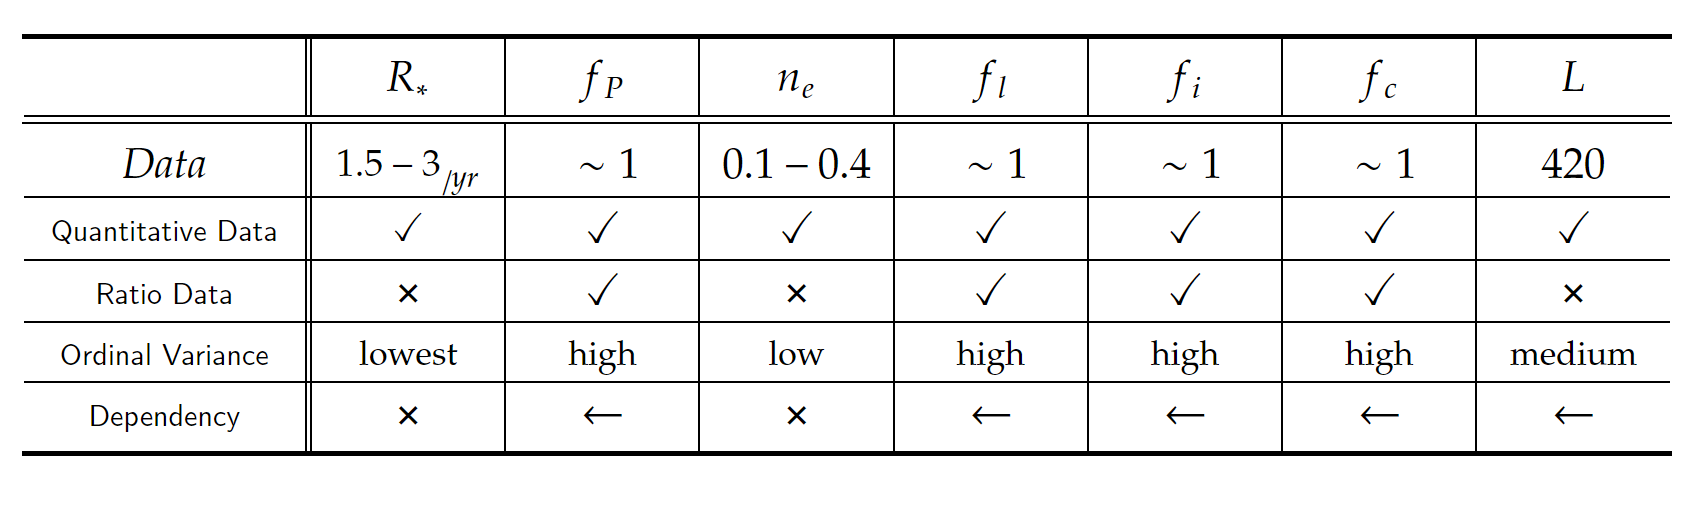
\includegraphics[width=0.96\linewidth]{table.png}
    \caption{Statistical characteristics of the parameters in the model.}
    \vspace{2em}
    \label{table}
\end{figure*}

\EOD
\end{document}
